\chapter{Derivatan}
Ett av de mest fundamentala koncepten inom matematisk analys är \underline{derivata}.
Handlar om hur snabbt en given funktion förändras i närheten av en punkt $x$.
Kan hämta inspiration från medelhastigheter.\\
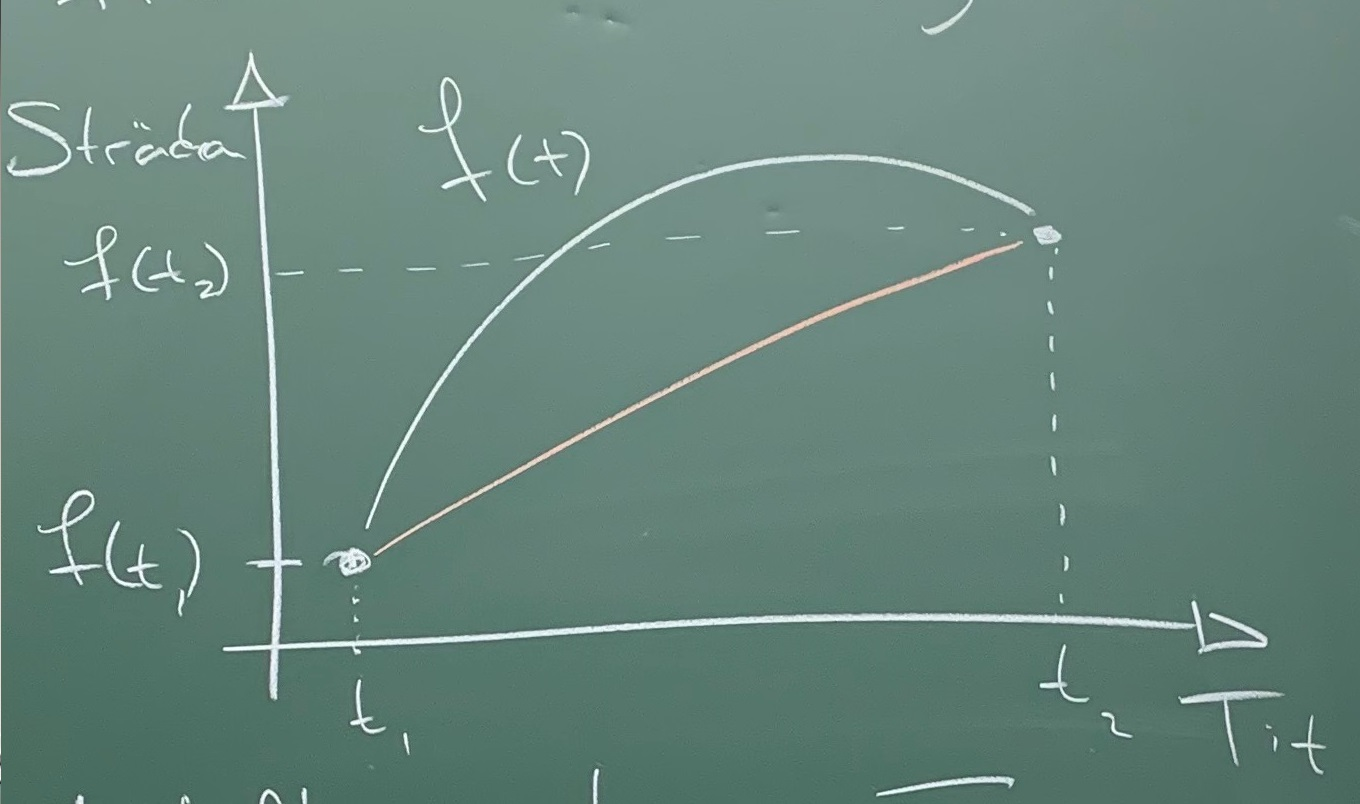
\includegraphics[scale=0.2]{lessons/lesson06/imgs/img01.jpg}\\
Medelhastigheten $\overline{v}$ mellan $t_1$ och $t_2$ är $\overline{v}=\frac{f(t_2)-f(t_1)}{t_2-t_1}$.
Just $\overline{v}$ är dessutom lutningen på den linje som går från $(t_1,f(t_1))$ till $t_2,f(t_2)$.
\begin{equation*}
    \overline{v}=\frac{y-f(t_1)}{x-t_1}\Leftrightarrow y=\overline{v}(x-t_1)+f(t_1)
\end{equation*}
Uppenbart att ju närmre $t_2$ är $t_1$ desto mer kan $\overline{v}$ tolkas som den momentana hastigheten i $t_1$
och "snittlinjen" övergår till att bli en tangent.\\
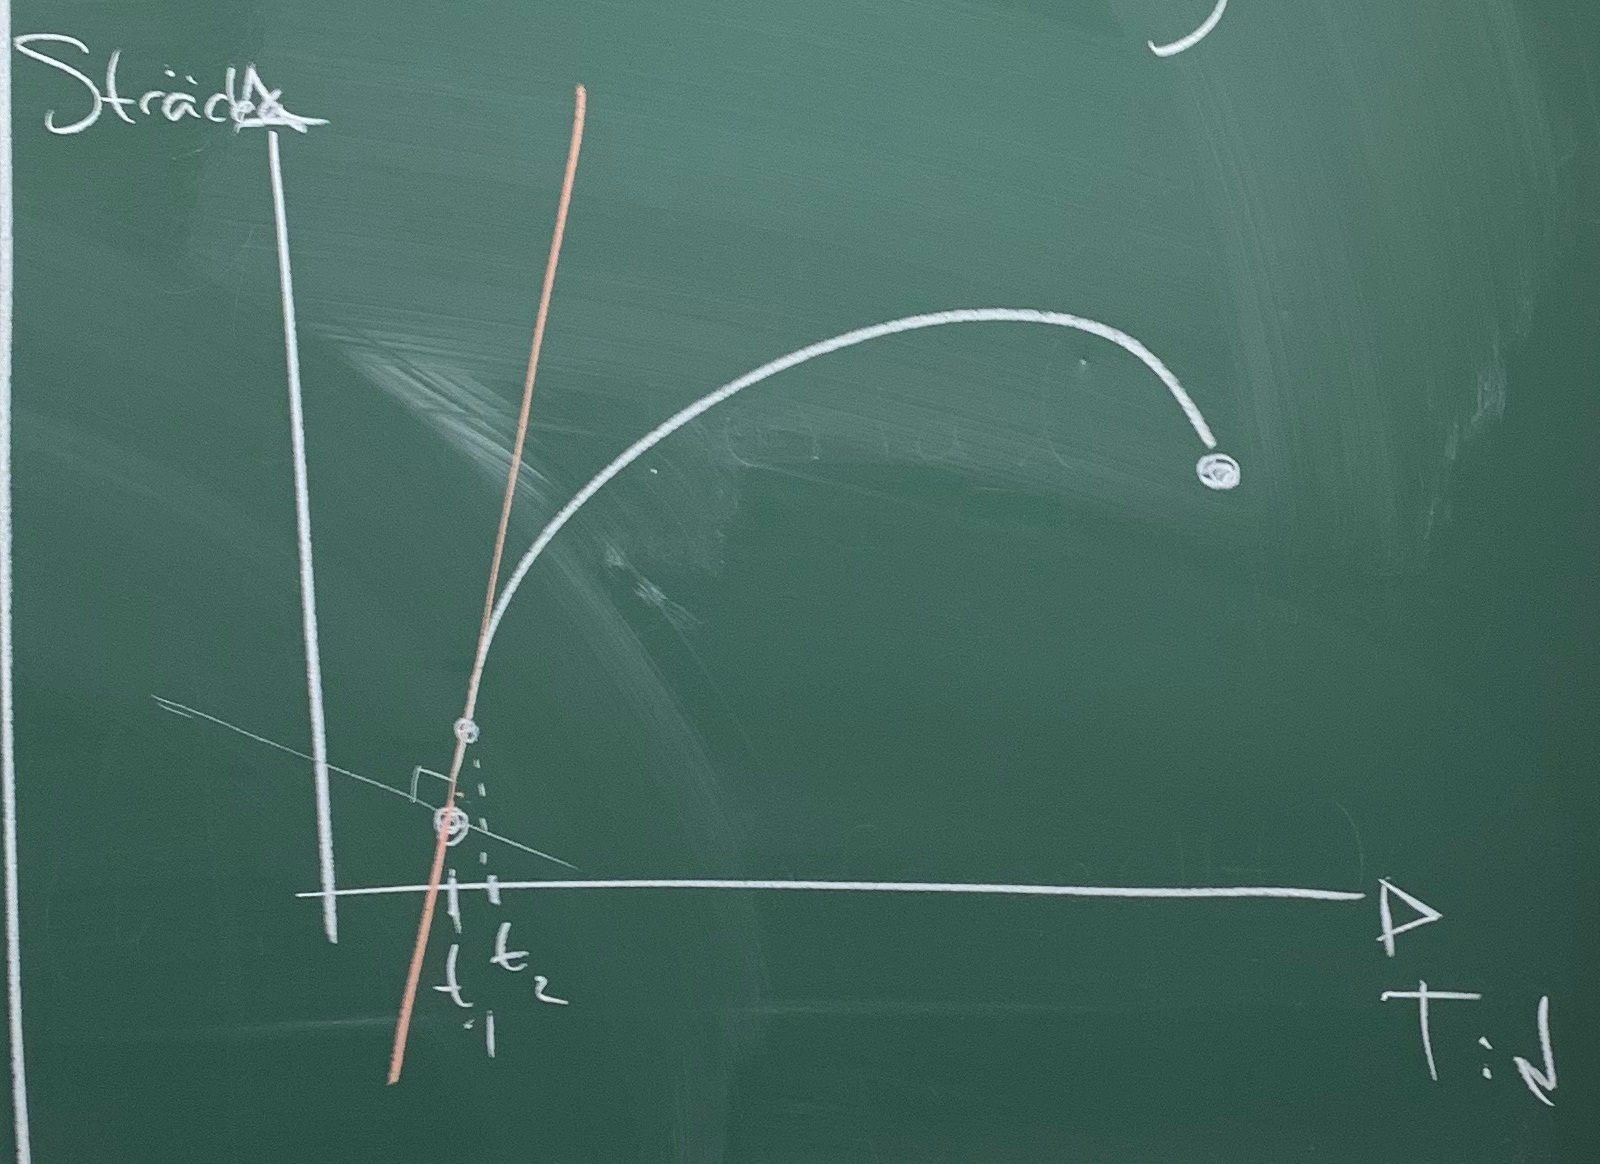
\includegraphics[scale=0.2]{lessons/lesson06/imgs/img02.jpg}\\
\\
Naturligt  att definiera den momentana hastigheten i en punkt $x_0$ för en given funktion $f$ som
\begin{equation*}
    \lim_{h\to 0}\frac{f(x_0+h)-f(x_0)}{(x_0+h)-x_0}=\lim_{h\to 0}\frac{f(x_0+h)-f(x_0)}{h}
\end{equation*}
Om detta gränsvärde existerar så kallas det för \underline{derivatan} av $f$ i $x=x_0$ och betecknas som $f^\prime(x_0)$.
Geometriskt så kan $f^\prime(x_0)$ tolkas som tangentlinjens lutning i $x=x_0$ för grafen till $f$.

Precis som för gränsvärden kan man definiera höger- och vänsterderivatan som:
\begin{equation*}
    f_+^\prime(x_0^+)=\lim_{h\to 0}\frac{f(x_0+h)-f(x_0)}{h}
\end{equation*}
\begin{equation*}
    f_-^\prime(x_0^-)=\lim_{h\to 0}\frac{f(x_0+h)-f(x_0)}{h}
\end{equation*}
En funktion $f$ sägs vara deriverbar på ett intervall $[a,b]$ om den är deriverbar i varje punkt $x\in[a,b]$
och höger- respektive vänsterderiverbar i $a$ respektive $b$.

från derivatan kan man enkelt beräkna lutningen för \underline{normalen}, dvs. den linjen som är vinkelrät mot tangenten som:
\begin{equation*}
    \text{Normalens lutning i }x_0=-\frac{1}{f^\prime(x_0)}
\end{equation*}
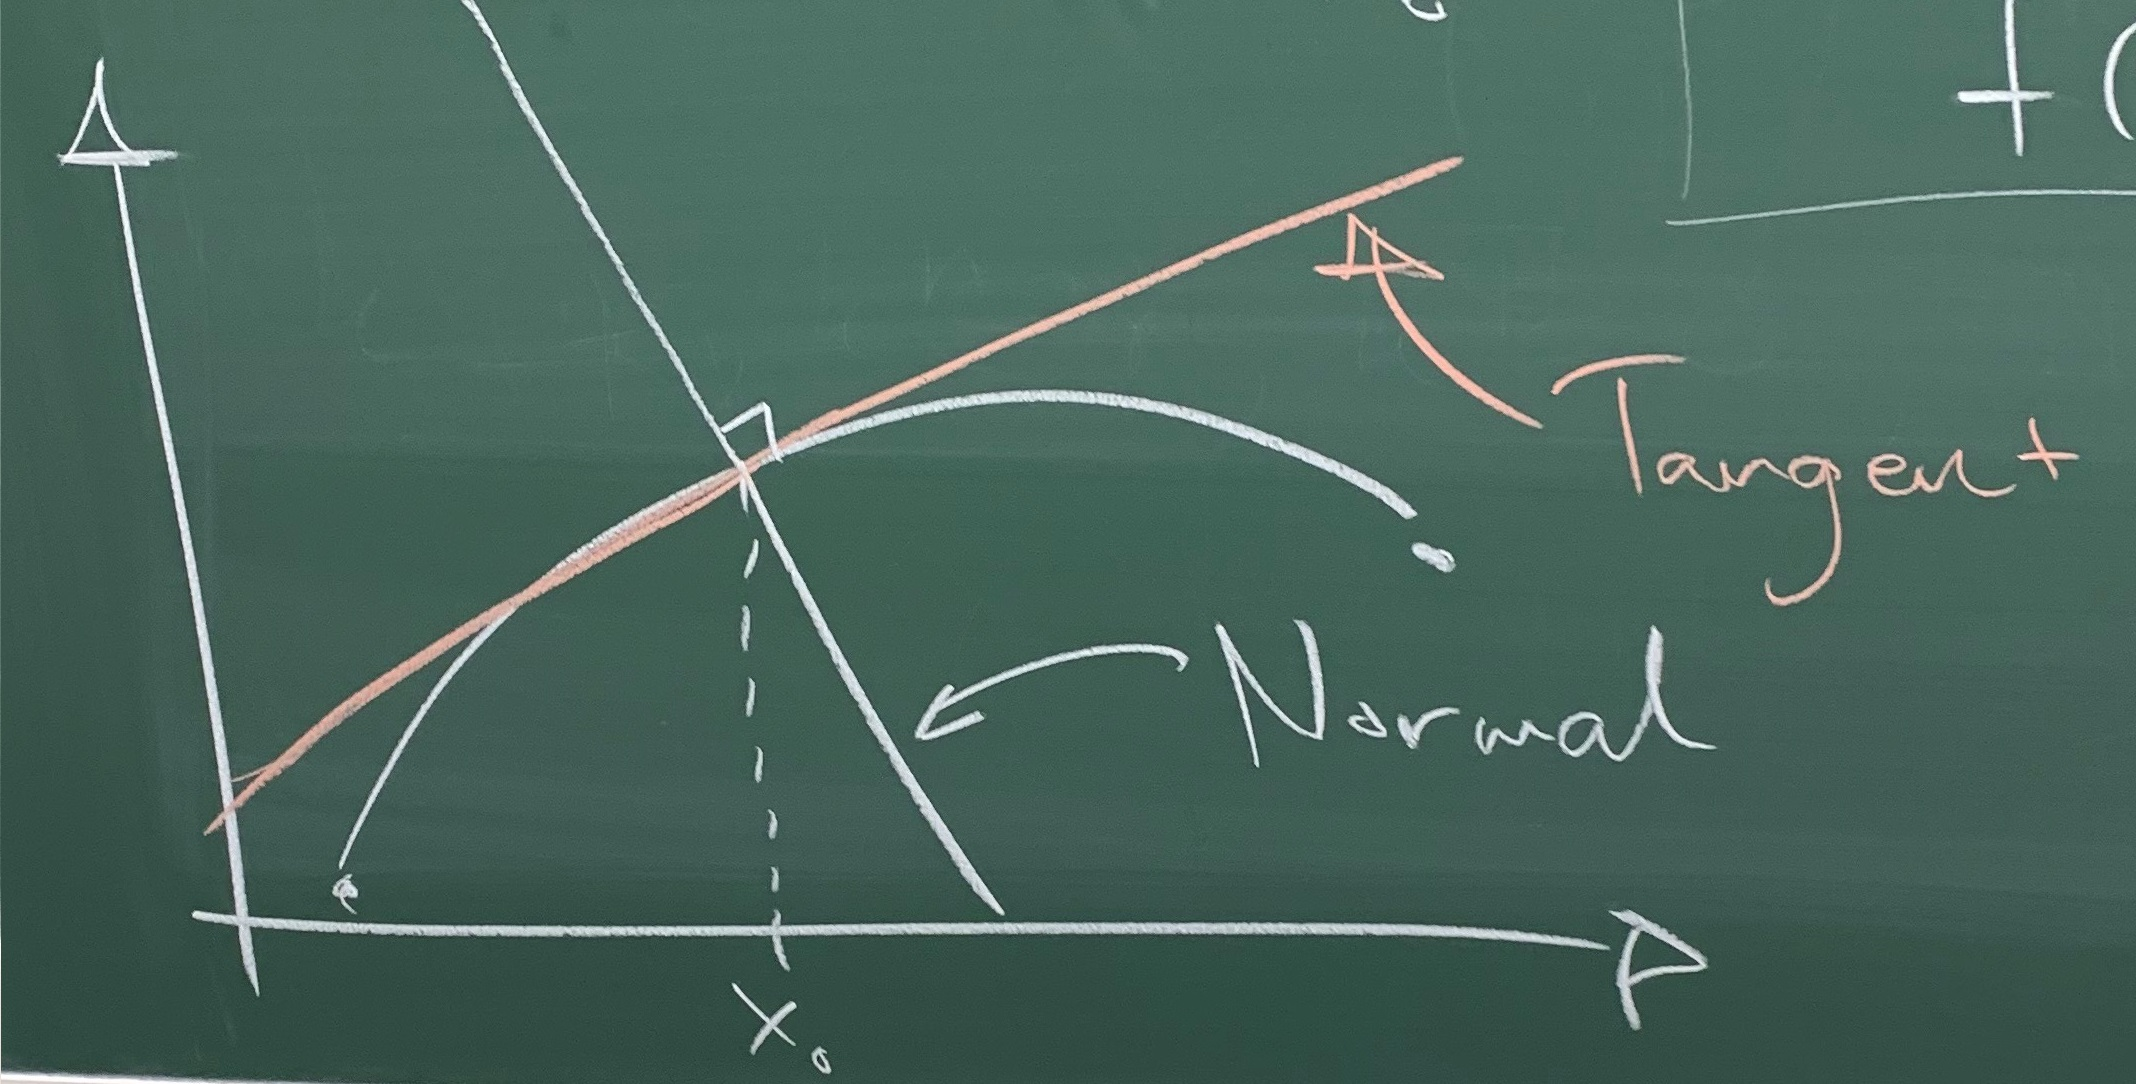
\includegraphics[scale=0.2]{lessons/lesson06/imgs/img03.jpg}

\paragraph{Ex}(2.2.21)\\
Använd derivatans definition och beräkna $f^\prime(x)$ givet funktionen $f(x)=\frac{1}{\sqrt{1+x^2}}$.
\subparagraph{Lösning}
Vi måste beräkna följande gränsvärde då $h\to 0$:
\begin{equation*}
    \frac{f(x+h)-f(h)}{h}=
    \frac{1}{\sqrt{1+(x+h)^2}}-\frac{1}{\sqrt{1+x^2}}=
    \frac{\frac{\sqrt{1+x^2}-\sqrt{1+(x+h)^2}}{\sqrt{1+(x+h)^2}\cdot\sqrt{1+x^2}}}{h}=
\end{equation*}
\begin{equation*}
    \frac{\sqrt{1+x^2}-\sqrt{1+(x+h)^2}}{h\sqrt{1+(x+h)^2}\sqrt{1+x^2}}\cdot\frac{\sqrt{1+x^2}+\sqrt{1+(x+h)^2}}{\sqrt{1+x^2}+\sqrt{1+(x+h)^2}}=
\end{equation*}
\begin{equation*}
    \frac{(1+x^2)-(1+(x+h)^2)}{h\sqrt{1+(x+h)^2}\sqrt{1+x^2}(\sqrt{1+x^2}+\sqrt{1+(x+h)^2})}=
\end{equation*}
\begin{equation*}
    \frac{1+x^2-(1+x^2+2xh+h^2)}{h\sqrt{1+(x+h)^2}\sqrt{1+x^2}(\sqrt{1+x^2}+\sqrt{1+(x+h)^2})}=
\end{equation*}
\begin{equation*}
    \frac{-h(2x+h)}{h\sqrt{1+(x+h)^2}\sqrt{1+x^2}(\sqrt{1+x^2}+\sqrt{1+(x+h)^2})}=
\end{equation*}
\begin{equation*}
    \frac{-2x-h}{\sqrt{1+(x+h)^2}\sqrt{1+x^2}(\sqrt{1+x^2}+\sqrt{1+(x+h)^2})}
\end{equation*}
Då $h\to 0$ får vi:
\begin{equation*}
    -\frac{2x}{\sqrt{1+x^2}\sqrt{1+x^2}(\sqrt{1+x^2}+\sqrt{1+x^2})}=
    -\frac{2x}{2(1+x^2)^3}=
    \frac{x}{(1+x^2)^(\frac{3}{2})}
\end{equation*}

\section{Räkneregler och standard derivator}
Några standard derivator:
\begin{itemize}
    \item $f(x)=c \Rightarrow f^\prime(x)=0$
    \item $f(x)=x^r \Rightarrow f^\prime(x)=r\cdot x^{r-1}$
    \item $f(x)=c \Rightarrow f^\prime(x)=0$
\end{itemize}
Genom derivatans definition visar amn enkelt att
\begin{itemize}
    \item $(f\pm g)^\prime(x)=f^\prime(x)\pm g^\prime(x)$
    \item $(c\cdot f)^\prime(x)=c \cdot f^\prime(x)$
\end{itemize}
Två andra \underline{extremt} viktiga räkneregler för derivator är produktregeln och kedjeregeln.
\paragraph{Produktregeln}
\begin{equation*}
    (f\cdot g)^\prime(x)=f^\prime(x)\cdot g(x)+f(x)\cdot g^\prime(x)
\end{equation*}
(Ur denna får man öven "kvotregeln" genom att sätta $\frac{f(x)}{g(x)}=f(x)\cdot g^{-1}(x)$)

\paragraph{Kedjeregeln}
\begin{equation*}
    (f\circ g)^\prime(x)=
    f(g(x))^\prime=
    f^\prime(g(x))\cdot g^\prime(x)
\end{equation*}
Kedjregeln ligger till grund för alla implementationer av träningssteget för neurala nätverk
(typ av AI agloritm) nämligen genom så kallad "backwards propogation".
\\\\
Intuitivt motsvarar derivatan $f^\prime(x)$ tangentlinjens lutning för $f$ i $x$.
Borde betyda att $f$ "hänger ihop" i $x$, dvs att $f$ är kontinuerlig i $x$?

\paragraph{Sats} Deriverbarhet ger kontinuitet (tenta)\\
Om $f$ är deriverbar i $x$ så är $f$ också kontinuerlig i $x$.
\subparagraph{Bevis} Att $f$ är deriverbar i $x$ betyder att gränsvärdet
$\lim_{h\to 0}\frac{f(x+h)-f(x)}{h}$ existerar.
Men det betyder att $\lim_{h\to 0}(f(x+h)-f(x))=\lim_{h\to 0}(f(x+h)-f(x)\frac{h}{h})=\lim_{h\to 0}\frac{f(x+h)-f(x)\cdot h}{h}=0$
så $\lim_{h\to 0}(f(x+h)-f(x))=0\Leftrightarrow\lim_{h\to 0}f(x+h)=f(x)$.
Låt $x+h=y\Rightarrow\lim_{y\to x}f(y)=f(x)$, dvs. $f$ är kontinuerlig i $x$. $\Box$

Gäller det motsatta, dvs. att om $f$ är kontinuerlig i $x$ så är $f$ deriverbar i $x$?
Nej! Till exempel är så kallade
\paragraph{Browask rörelse} B(t) (slumpfunktion)
Kontinuerlig i alla punkter men ej deriverbar någonstans.
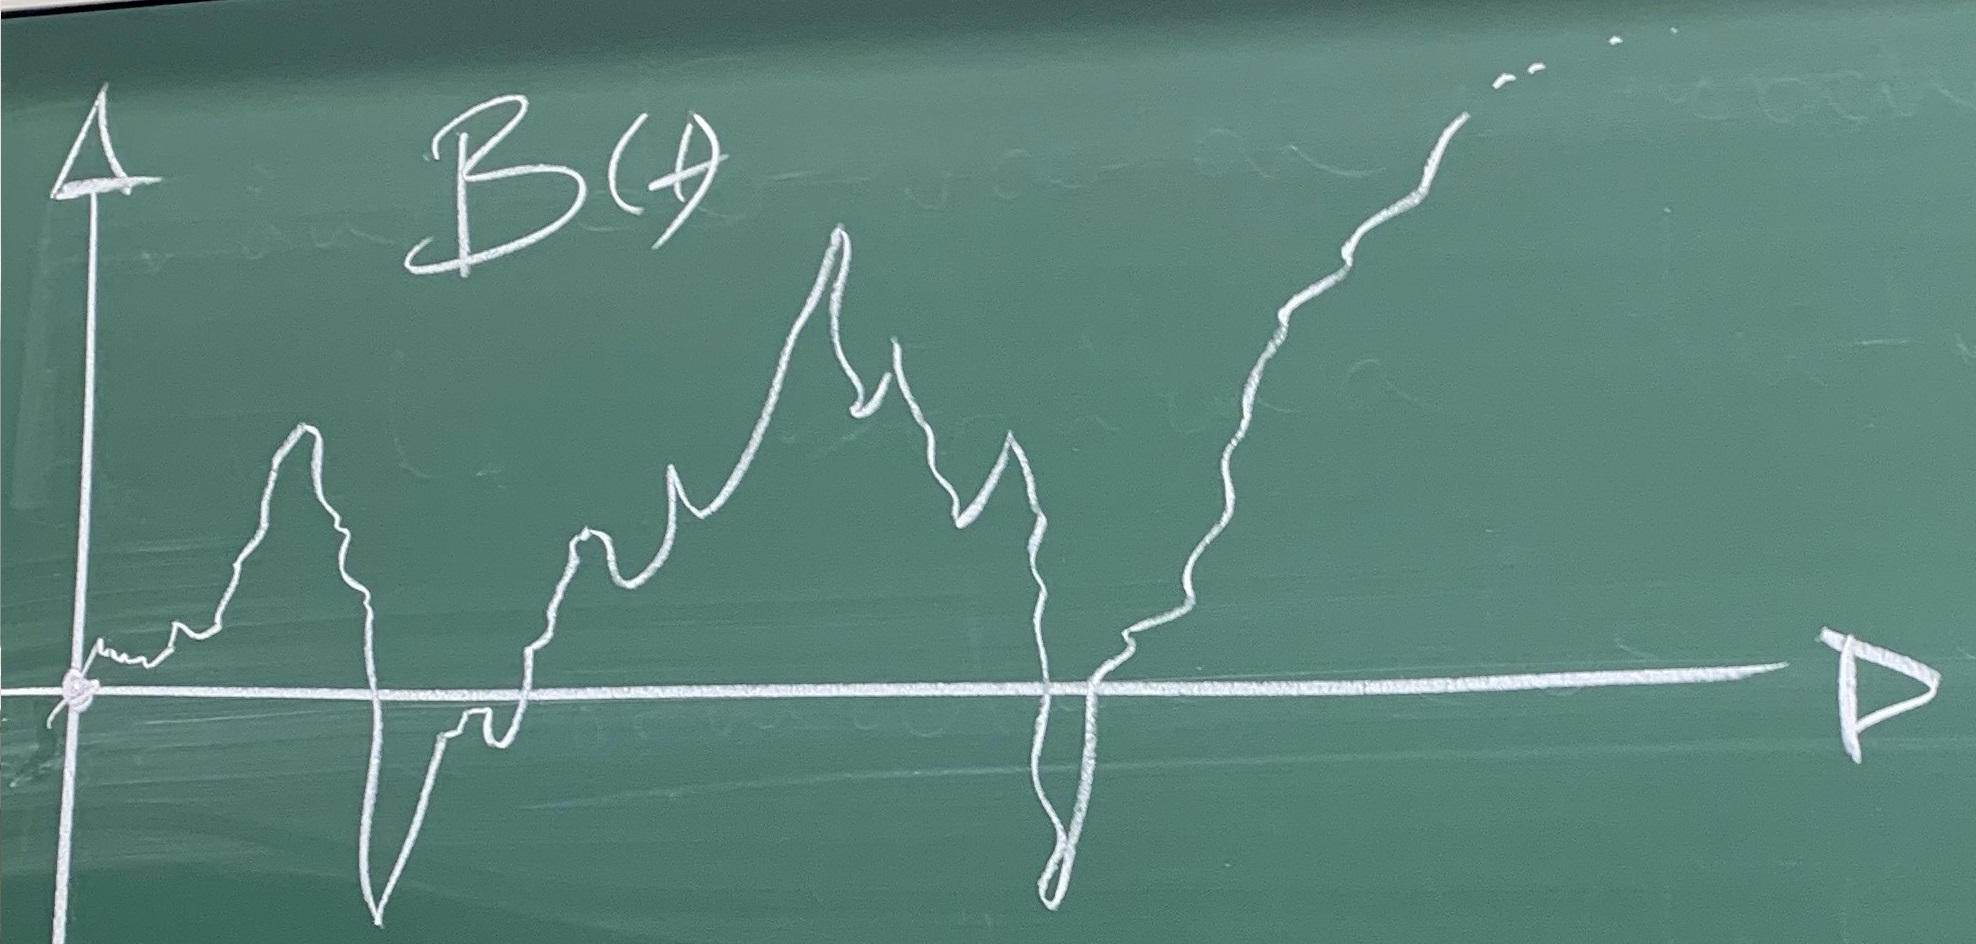
\includegraphics[scale=0.2]{lessons/lesson06/imgs/img04.jpg}\\
Browask rörelse används bland annat inom signalbehandling och inom
matematisk finans (för att modellera aktieprisutveckling).

\paragraph{Derivatan av trigonometriska funktioner}
\begin{itemize}
    \item $\frac{d}{dx}sin(x)=cos(x)$
    \item $\frac{d}{dx}cos(x)=-sin(x)$
    \item $\frac{d}{dx}tan(x)=\frac{1}{cos^2(x)}=\frac{1}{1-sin^2(x)}=\{\frac{cos^2(x)+sin^2(^x)}{cos^2(x)}\}=1+tan^2(x)$
\end{itemize}
Alla dessa bygger på beviset att $\lim_{x\to 0}\frac{sin(x)}{x}=1$

\paragraph{Ex} (2.4.12)
Beräkna derivatan av $f(x)=(2+|x|^3)^{\frac{1}{3}}$.
\subparagraph{Lösning}
Tänk på $2+|x|^3$ som en inre funktion och använd kedjeregeln!
\begin{equation*}
    f^\prime(x)=\frac{1}{3}\cdot (2+|x|^3)^{\frac{1}{3}-1}\cdot(2+|x|^3)^\prime=
    \frac{1}{3}(2+|x|^3)^{-\frac{2}{3}}\cdot(2+|x|^3)^\prime
\end{equation*}
Vad är derivatan av $2+|x|^3$?
\begin{equation*}
    (2+|x|^3)^\prime=0+(|x|^3)^\prime=
    3\cdot|x|^2\cdot(|x|)^\prime
\end{equation*}
Vad är $(|x|)^\prime$?
\begin{equation*}
    |x|=\left\lbrace\begin{matrix}
        x\text{, om } x\geq 0 \\
        -x\text{, om} x < 0
    \end{matrix}\right.
    \Rightarrow
    \underbrace{(|x|)^\prime=\left\lbrace\{\begin{matrix}
            1\text{, om } > 0 \\
            -1\text{, om } < 0
        \end{matrix}\right.}
\end{equation*}
$=sgn(x) \text{(sign function)}$

så $f^\prime(x)=\frac{1}{3}(2+|x|^3)^\frac{-2}{3}\cdot 3\cdot|x|^3\cdot sgn(x)=
    \frac{x^2}{(2+|x|^3)^\frac{2}{3}}\cdot sgn(x),x\neq 0$